\documentclass{article} 
\usepackage[landscape]{geometry}
\usepackage{tikz}
\usetikzlibrary{mindmap}
\usepackage{dtklogos}
\begin{document}
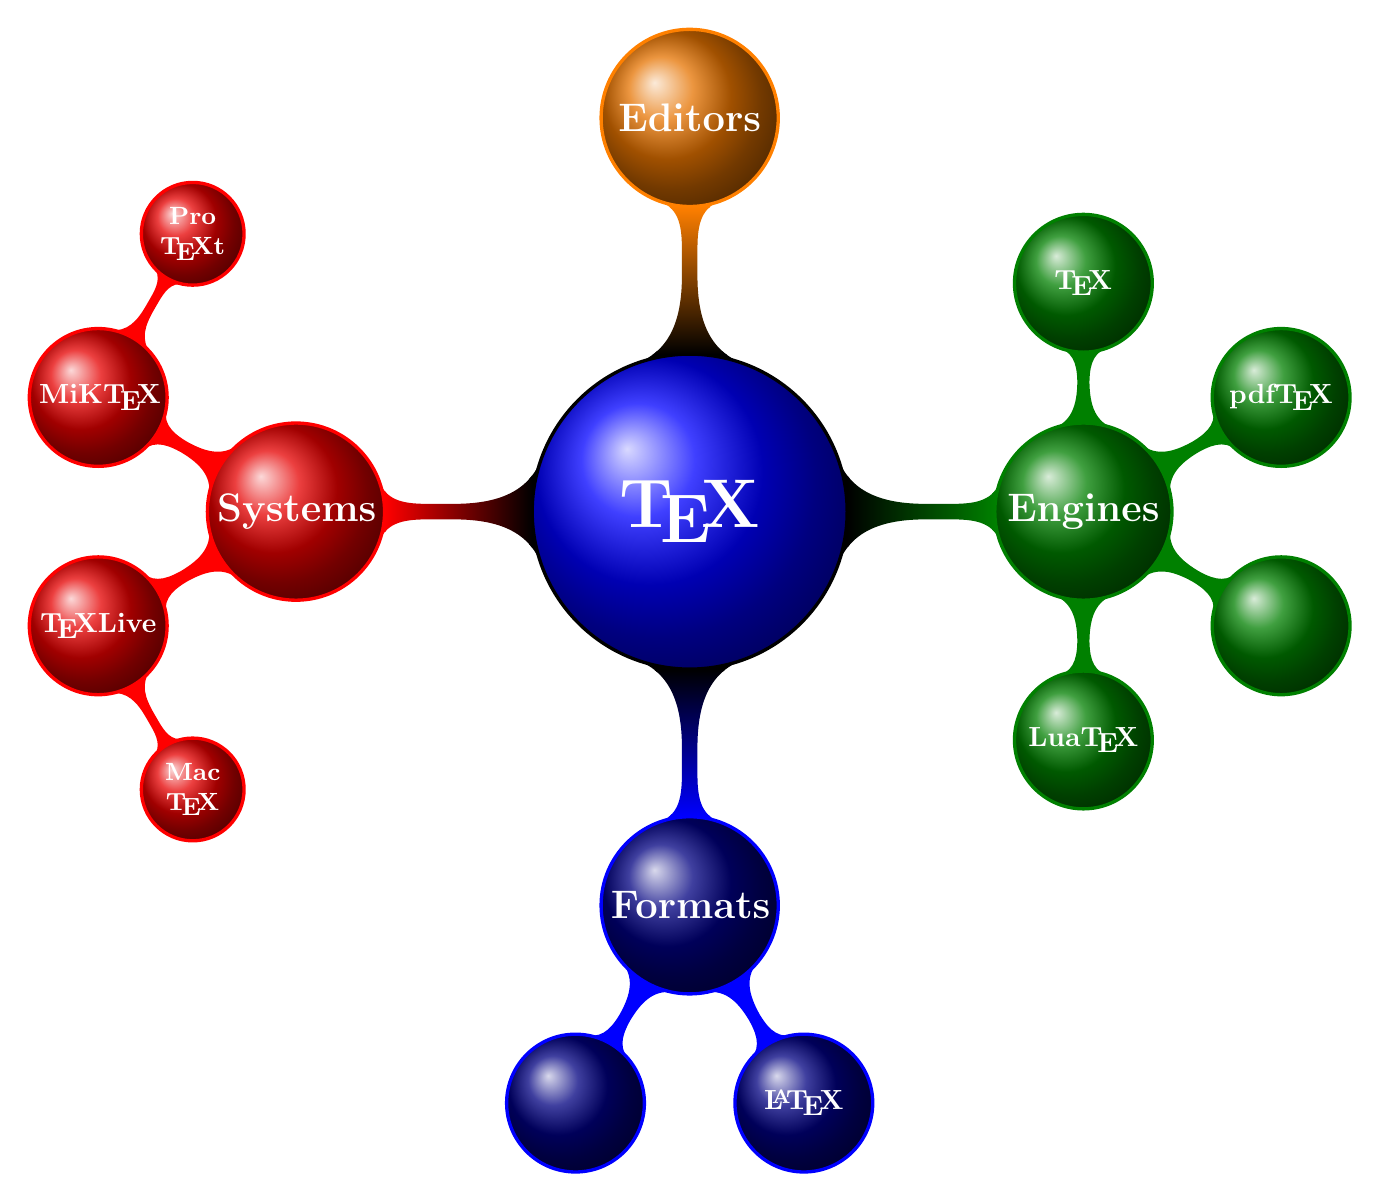
\begin{tikzpicture}
  \path [
    mindmap,
    text = white,
    level 1 concept/.append style =
      {font=\Large\bfseries, sibling angle=90},
    level 2 concept/.append style =
      {font=\normalsize\bfseries},
    level 3 concept/.append style =
      {font=\small\bfseries},
    tex/.style     = {concept, ball color=blue,
      font=\Huge\bfseries},
    engines/.style = {concept, ball color=green!50!black},
    formats/.style = {concept, ball color=blue!50!black},
    systems/.style = {concept, ball color=red!90!black},
    editors/.style = {concept, ball color=orange!90!black}
  ]
  node [tex] {\TeX} [clockwise from=0]
    child[concept color=green!50!black, nodes={engines}] {
      node {Engines} [clockwise from=90]
        child { node {\TeX} }
        child { node {pdf\TeX} }
        child { node {\XeTeX} }
        child { node {Lua\TeX} }}
    child [concept color=blue, nodes={formats}] {
      node {Formats} [clockwise from=300]
        child { node {\LaTeX} }
        child { node {\ConTeXt} }}
    child [concept color=red, nodes={systems}] {
      node {Systems} [clockwise from=210]
        child { node {\TeX Live} [clockwise from=300]
          child { node {Mac \TeX} }}
        child { node {MiK\TeX} [clockwise from=60]
          child { node {Pro \TeX t} }}}
    child [concept color=orange, nodes={editors}] {
      node {Editors} };
\end{tikzpicture}
\end{document}